Le jeu de donné utilisé comporte 360 feuilles en images couleur et noir et blanc réparties et triées en 36 espèces. Le nombres d'individu par groupe est assez réduit et ne dépasse pas le nombre de 16. Une imprécision peut donc apparaitre dû au nombre réduit d'individu dans chaque échantillon.
\paragraph{}
Les images ont une résolution de 960*720 pixel, ce qui offre précision suffisante, sans être excessive. Cependant le temps de calcul pour la sérialisation des données reste assez long : quelques secondes par image. Une sauvegarde de celle-ci est donc fortement conseillée.
\paragraph{}
La représentation des feuilles est homogène : l'image est centrée et pour chaque feuille le pétiole est placé vers le bas de l'image, ce qui permet de faciliter grandement le traitement de l'image dans la mesure ou aucune rotation n'est nécessaire en pré-traitement.

\begin{center}
	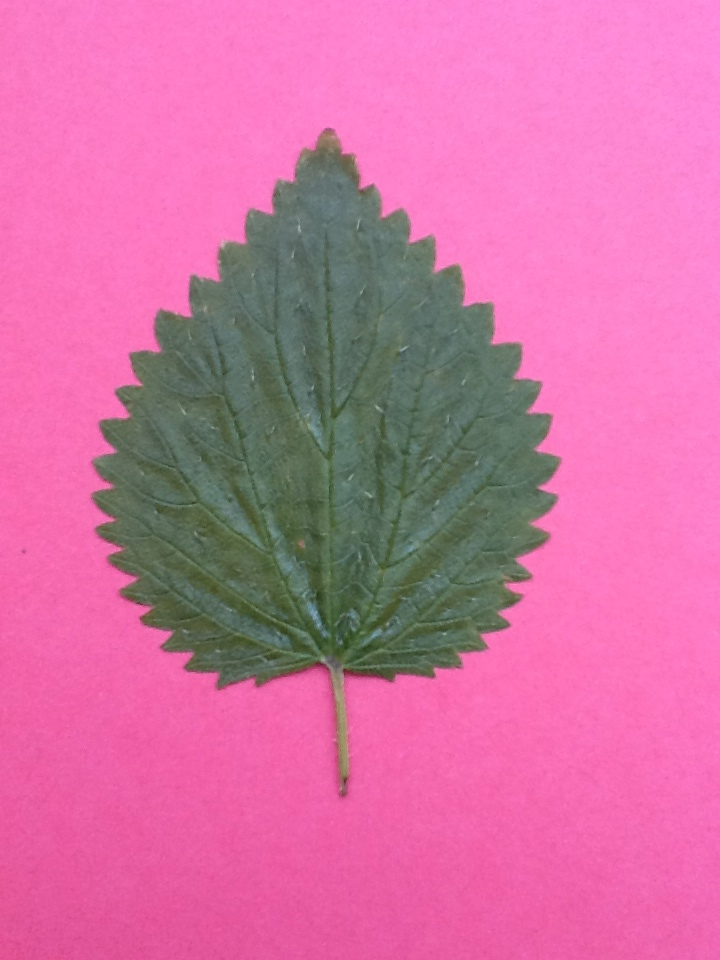
\includegraphics[scale=0.11]{image/urticaRGB.png}	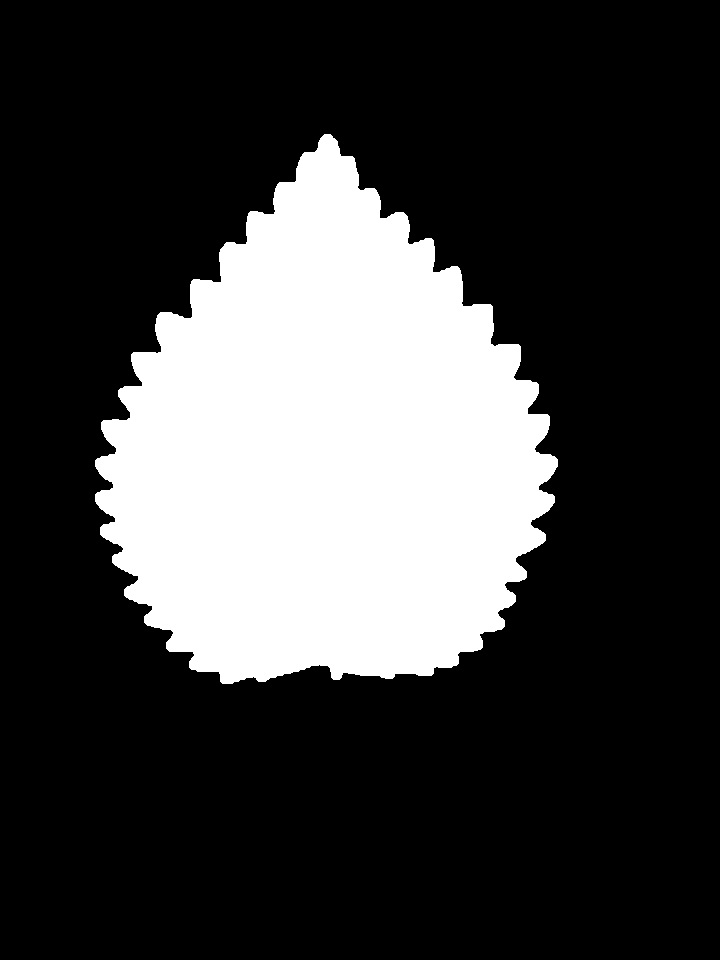
\includegraphics[scale=0.15]{image/urticaNB.png}
\end{center}